\documentclass{article}
\usepackage{multicol}
\usepackage{listings}
\usepackage{color}
\usepackage{makecell}
\usepackage{cprotect}
\usepackage{graphicx}
\usepackage{amssymb}
\usepackage{commath}
\usepackage{amsthm}
\usepackage{amsfonts}
\usepackage{wasysym}

\definecolor{mygreen}{rgb}{0,0.6,0}
\definecolor{mygray}{rgb}{0.5,0.5,0.5}
\definecolor{mymauve}{rgb}{0.58,0,0.82}
 
%Customize a bit the look
\lstset{ %
backgroundcolor=\color{white}, % choose the background color; you must add \usepackage{color} or \usepackage{xcolor}
basicstyle=\footnotesize, % the size of the fonts that are used for the code
breakatwhitespace=false, % sets if automatic breaks should only happen at whitespace
breaklines=true, % sets automatic line breaking
captionpos=b, % sets the caption-position to bottom
commentstyle=\color{mygreen}, % comment style
deletekeywords={...}, % if you want to delete keywords from the given language
escapeinside={\%*}{*)}, % if you want to add LaTeX within your code
extendedchars=true, % lets you use non-ASCII characters; for 8-bits encodings only, does not work with UTF-8
frame=single, % adds a frame around the code
keepspaces=true, % keeps spaces in text, useful for keeping indentation of code (possibly needs columns=flexible)
keywordstyle=\color{blue}, % keyword style
% language=Octave, % the language of the code
morekeywords={*,...}, % if you want to add more keywords to the set
numbers=left, % where to put the line-numbers; possible values are (none, left, right)
numbersep=5pt, % how far the line-numbers are from the code
numberstyle=\tiny\color{mygray}, % the style that is used for the line-numbers
rulecolor=\color{black}, % if not set, the frame-color may be changed on line-breaks within not-black text (e.g. comments (green here))
showspaces=false, % show spaces everywhere adding particular underscores; it overrides 'showstringspaces'
showstringspaces=false, % underline spaces within strings only
showtabs=false, % show tabs within strings adding particular underscores
stepnumber=1, % the step between two line-numbers. If it's 1, each line will be numbered
stringstyle=\color{mymauve}, % string literal style
tabsize=2, % sets default tabsize to 2 spaces
title=\lstname % show the filename of files included with \lstinputlisting; also try caption instead of title
}
%END of listing package%
 
\definecolor{darkgray}{rgb}{.4,.4,.4}
\definecolor{purple}{rgb}{0.65, 0.12, 0.82}
 
%define Javascript language
\lstdefinelanguage{JavaScript}{
keywords={typeof, new, true, false, catch, function, return, null, catch, switch, var, if, in, while, do, else, case, break},
keywordstyle=\color{blue}\bfseries,
ndkeywords={class, export, boolean, throw, implements, import, this},
ndkeywordstyle=\color{darkgray}\bfseries,
identifierstyle=\color{black},
sensitive=false,
comment=[l]{//},
morecomment=[s]{/*}{*/},
commentstyle=\color{purple}\ttfamily,
stringstyle=\color{red}\ttfamily,
morestring=[b]',
morestring=[b]"
}
 
\lstset{
language=JavaScript,
extendedchars=true,
basicstyle=\footnotesize\ttfamily,
showstringspaces=false,
showspaces=false,
numbers=left,
numberstyle=\footnotesize,
numbersep=9pt,
tabsize=2,
breaklines=true,
showtabs=false,
captionpos=b
}

\setlength{\parindent}{0pt}
\newtheorem{theorem}{Teorema}[section]
\newtheorem{lemma}{Lemma}[section]
\newtheorem{corollary}{Corollario}[section]

\title{Progammazione e Algoritmica}
\author{Angelo Passarelli}
\date{\today}

\renewcommand*\contentsname{Sommario}
\renewcommand\qedsymbol{$\blacksquare$}
\renewcommand*{\proofname}{Dimostrazione}

\begin{document}

\maketitle

\tableofcontents

\pagebreak

\section{Algoritmi di Ordinamento}

\subsection{Analisi Complessità}

\begin{center}
    \begin{tabular}{|c|c|c|c|}
        \hline
        & \multicolumn{3}{c|}{Complessità} \\
        \hline
        Algoritmo & Caso Migliore & Caso Peggiore & Caso Medio \\ \hline
        Insertion Sort & $O(n)$ & $O(n^2)$ & $O(n^2)$ \\ \hline
        Selection Sort & $O(n^2)$ & $O(n^2)$ & $O(n^2)$ \\ \hline
        Merge Sort & $\Theta(n \log n)$ & $\Theta(n \log n)$ & $\Theta(n \log n)$ \\ \hline
        QuickSort & $\Theta(n \log n)$ & $\Theta(n^2)$ & $\Theta(n \log n)$ \\ \hline
        HeapSort & $O(n \log n)$ & $O(n \log n)$ & $O(n \log n)$ \\ \hline
        Counting Sort & $O(max\{n, k\})$ & $O(max\{n, k\})$ & $O(max\{n, k\})$ \\ \hline
        Radix Sort & $O(d(n + k))$ & $O(d(n + k))$ & $O(d(n + k))$ \\ \hline       
    \end{tabular}
\end{center}

\subsection{Insertion Sort}

\subsubsection{Descrizione}

\begin{enumerate}
    \item All'inizio dell'algoritmo l'insieme ordinato è vuoto (\verb|[]|).
    \item Il primo elemento dell'array (\verb|A[0]|) risulta già ordinato rispetto alla sottosequenza che prendiamo in considerazione (infatti il \verb|for| parte da \verb|j = 1|).
    \item L'elemento successivo (\verb|key|) viene confrontato dall'elemento precedente a \verb|j| fino all'ultima cella dell'array, solo fino a quando \verb|key| risulta più piccolo dei sui elementi precedenti.
    \item Nel caso in cui \verb|key| deve occupare la cella già occupata da un altro elemento, occorre shiftare tutti gli elementi più grandi di \verb|key| alla sua destra (riga \verb|6|).
    \item Si ripete dal punto \verb|3.| per tutti gli \verb|n| elementi.
\end{enumerate}

\subsubsection{Invariante di Ciclo}

All'inizio, durante e alla fine del ciclo \verb|for| la porzione dell'array \verb|[0, j-1]| risulta ordinata.

\lstinputlisting[language=JavaScript]{code/insertion.js}

\subsection{Selection Sort}

\subsubsection{Descrizione}

\begin{enumerate}
    \item Si cerca il minimo dell'array nella sottoporzione \verb|[i, n-1]| con \verb|i| che parte da \verb|0|.
    \item Alla fine della ricerca, l'elemento minimo viene posto all'inizio della sottoporzione.
    \item Si ritorno al punto \verb|1.| fino a \verb|n-1|.
\end{enumerate}

\subsubsection{Invariante di Ciclo}

All'inizio, durante e alla fine del primo ciclo \verb|for| la porzione dell'array \verb|[0, i]| risulta ordinata.

\lstinputlisting[language=JavaScript]{code/selection.js}

\subsection{Merge Sort}

\subsubsection{Descrizione}

\begin{enumerate}
    \item L'array viene prima diviso in 2 parti ricorsivamente fino a quando la sottoporzione da dividere non raggiunge dimensione 1.
    \item Successivamente, a partire dall'ultima scomposizione (quindi all'inizio avremo tutte le celle di lunghezza 1 che per definizione sono già ordinate) viene effettuata la procedura di \verb|Merge()| che prende due porzioni di array già ordinate e le fonde in un unico array in modo da mantenere l'ordinamento.
\end{enumerate}

\cprotect\subsubsection{Descrizione \verb|Merge()|}

\begin{enumerate}
    \item All'inizio vengono prima calcolate le dimensioni delle 2 sottosequenze.
    \item Successivamente vengono creati due array di appoggio dove saranno copiati i valori delle 2 sottoporzioni.
    \item Nell'ultima cella dei due array di appoggio viene posto un valore sentinella (in questo caso $+ \infty$) in modo tale che quando avremo terminato di inserire nell'array principale i valori di una delle due sottosequenze, potremo continuare a copiare gli elementi dell'altra sottoporzione in modo corretto dato che verranno sempre confrontati con $+ \infty$.
    \item L'idea di base del \verb|Merge()| si trova all'interno del ciclo \verb|for|. Infatti i due array essendo già ordinati, per trovare il valore più piccolo della loro unione basterà confrontare i valori minimi corrispettivi che all'inizio si troveranno nella cella \verb|0|.
    \item Nel caso in cui il valore minimo si trovi in \verb|L|, il suo valore sarà copiato in \verb|A[k]| (con \verb|k| che parte da \verb|p|) e l'indice corrispondente a \verb|L| sarà incrementato di 1, invece se il valore minimo è contenuto in \verb|R|, l'indice incrementato sarà \verb|j|.
    \item Quindi alla fine di ogni ciclo \verb|for| saranno sempre confrontati gli elementi più piccoli dei due array che non sono stati ancora copiati in \verb|A|.
    \item Il ciclo termina quando vengono copiati tutti gli \verb|r| elementi. In questo modo preveniamo anche che non vengano copiati i valori sentinella.
\end{enumerate}

\subsubsection{Invariante di Ciclo}

All'inizio di ogni iterazione del \verb|for| il sottorray \verb|A[p...k-1]| contiene i \verb|k-p| elementi più piccoli di \verb|L| e \verb|R| già ordinati. \\
Inoltre \verb|L[i]| e \verb|R[j]| contengono i più piccoli elementi che non sono stati ancora copiati in \verb|A|. 

\lstinputlisting[language=JavaScript]{code/merge.js}

\subsection{QuickSort}

\subsubsection{Descrizione}

\begin{enumerate}
    \item Viene scelto un elemente chiamato \verb|pivot| (nel codice \verb|q|) e vengono spostati a sinistra tutti gli elementi di piccoli del \verb|pivot| e a destra tutti gli elementi più grandi (funzione \verb|Partiziona()|).
    \item Successivamente viene richiamato il \verb|QuickSort()| ricorsivamente sulla partizione a sinistra del \verb|pivot| e su quella a destra.
\end{enumerate}

\cprotect\subsubsection{Descrizione \verb|Partiziona()|}

\begin{enumerate}
    \item Come \verb|pivot| viene scelto \verb|x| che rappresenta l'ultima cella della sottoporzione.
    \item Il funzionamento si base su due indici \verb|i| e \verb|j|, in modo tale che alla fine tra \verb|p| e \verb|i| avremo gli elementi più piccoli di \verb|x| e tra \verb|i+1| e \verb|j| avremo i più grandi.
    \item In questo modo, nel ciclo \verb|for| ogni volta che troviamo un elemento minore di \verb|x| incrementiamo di $1$ la dimensione della sottosequenza \verb|[p, i]| e ci spostiamo l'elemento in considerazione nell'ultima posizione.
    \item Al termine del \verb|for| scambiamo il \verb|pivot| con il primo degli elementi più grandi di esso e restituiamo la posizione del \verb|pivot|.
    \item In questo modo il l'elemento corrispondente al \verb|pivot| si troverà nella posizione corretta per ottenere l'array ordinato.
\end{enumerate}

\subsubsection{Invariante di Ciclo}

All'inizio di ogni iterazione del \verb|for| preso qualsiasi indice \verb|k| della sottoporzione:

\begin{itemize}
    \item Se \verb|p| $\leq$ \verb|k| $\leq$ \verb|i|, allora \verb|A[k]| $\leq$ \verb|x|.
    \item Se \verb|i+1| $\leq$ \verb|k| $\leq$ \verb|j-1|, allora \verb|A[k]| $>$ \verb|x|.
    \item Se \verb|k| $=$ \verb|r|, allora \verb|A[k]| $=$ \verb|x|.
\end{itemize}

Gli indici tra \verb|j| e \verb|r-1| non ci interessano perchè sono ancora da confrontare.

\subsubsection{Costo}

Il costo del \verb|QuickSort()| dipende dal bilanciamento delle 2 sottoporzioni. \\
Infatti se il \verb|pivot| si trova sempre al centro della sottosequenza allora la complessità sarà $\Theta(n \log n)$ (caso migliore). \\
Invece il caso peggiore si verifica quando \verb|Partiziona()| produce una sottosequenza lunga \verb|n-1| e l'altra quindi lunga \verb|0|. \\
In questo caso la complessità è uguale a $\displaystyle \sum_{i = 1}^n (n - i) = \Theta(n^2)$.

\subsubsection{Dimostrazione Costo al Caso Medio}

\begin{itemize}
    \item Per randomizzare la procedura devo fare in modo che il \verb|pivot| venga scelto in modo casuale tra \verb|p| ed \verb|r|.
    \item Definiamo due eventi con la stessa probabilità che possano verificarsi: ovvero che il \verb|pivot| finisca nella zona esterna della sequenza o che finisca nella zona interna.
    \begin{figure}[h]
        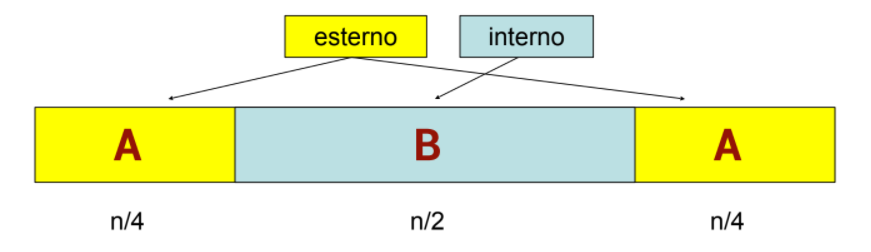
\includegraphics[scale=0.6]{img/random_pivot.png}
        \centering
    \end{figure}
    \item Nel caso in cui il \verb|pivot| finisca nella zona esterna, il caso peggiore si verifica quando esso si trova nella prima posizione, nel caso della sezione gialla di sinistra, o nell'ultima nel caso di quella di destra.
    \item Quindi in questo caso la complessità sarà: $T(n) = T(n - 1) + O(n)$.
    \item Invece, nel caso in cui il \verb|pivot| finisca nella zona interna, il caso peggiore si verifica quando esso si trova o all'inizio di \verb|B| quindi in posizione $\frac{n}{4}$ o alla fine di \verb|B|, in posizione $\frac{3}{4}n$.
    \item Quindi la complessità dell'algoritmo al caso peggiore sarà: $T(n) = T(n/4) + T(3/4 \; n) + O(n)$.
    \item Adesso occorre combinare la situazione \verb|A| con \verb|B|, e dato che, come già detto, hanno la stessa probabilità di verificarsi:
    \begin{equation*}
        \begin{split}
            T(n) & \leq A/2 + B/2 = \frac{1}{2}(A + B) \\
            & = \frac{1}{2}[T(n - 1) + T(n/4) + T(3/4 \; n) + O(n)] \\
            & \leq \frac{1}{2}[T(n) + T(n/4) + T(3/4 \; n) + O(n)] \\
        \end{split}     
    \end{equation*}
    \item Adesso moltiplico per $2$ a destra e a sinistra e porto il \verb|T(n)| nel secondo membro nel primo:
    \begin{equation*}
        \begin{split}
            2T(n) & \leq T(n) + T(n/4) + T(3/4 \; n) + O(n) \\
            T(n) & \leq T(n/4) + T(3/4 \; n) + O(n) \\
        \end{split}     
    \end{equation*}
    \item Ora per risolvere questa equazione utilizziamo l'albero di ricorrenza:
    \begin{figure}[h]
        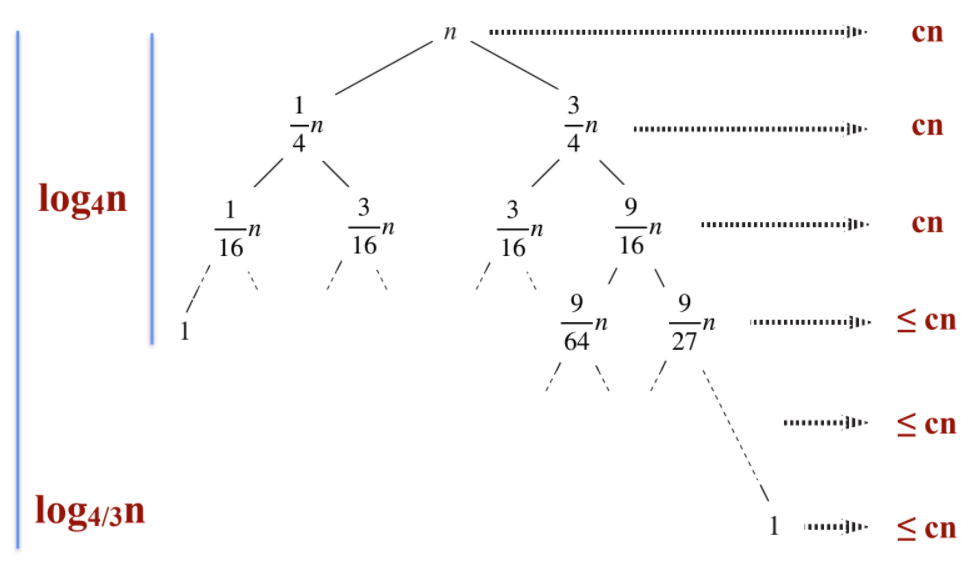
\includegraphics[scale=0.5]{img/albero_quicksort.png}
        \centering
    \end{figure}
    \item Qui possiamo notare come l'altezza del ramo più a sinistra sarà $\log_4 n$ mentre quella del ramo più a destra è $\log_{\frac{4}{3}} n$.
    \item Inoltre possiamo dire che se facciamo la somma dei nodi su ogni livello, fino a quando ogni livello è completo, questa sarà sempre uguale a $cn$.
    \item Invece dal livello in cui l'albero inizia a diventare sbilenco, fino all'ultimo livello, possiamo limitare superiormente la somma sempre con $cn$.
    \item Quindi in conclusione possiamo dire che la complessità del \verb|QuickSort()| al caso medio è $O(n \log n)$.
\end{itemize}

\lstinputlisting[language=JavaScript]{code/quicksort.js}

\subsection{HeapSort}

\subsubsection{Descrizione}

\begin{itemize}
    \item L'\verb|HeapSort()| si basa su una struttura dati chiamata Heap, ovvero un albero binario quasi completo, quindi dove tutti i livelli tranne l'ultimo sono completi e le foglie sull'ultimo livello vengono inserite da sinistra a destra.
    \item L'implementazione dell'Heap avviene tramite un array, in questo modo dato un nodo interno di indice \verb|i|, il figlio a sinistra si trova in posizione $2 \cdot i$ e quello a destra in $(2 \cdot i) + 1$ (se l'array parte da 1, nel caso dovesse partire da 0 il figlio a sinistra si troverebbe in posizione $(2 \cdot i) + 1$, mentre quello a destra in $(2 \cdot i) + 2$).
    \item Invece il genitore di \verb|i| si trova in posizione $\lfloor \frac{i - 1}{2} \rfloor$.
    \item Nell'array la prima foglia si trova in posizione $\frac{n}{2}$.
\end{itemize}

\cprotect\subsubsection{Descrizione \verb|Max_Heapify()|}

\begin{itemize}
    \item L'idea della procedura di \verb|Max_Heapify()| è quella di avere un albero con radice \verb|i| dove il sottoalbero sinistro e il sottoalbero destro sono già degli alberi di Max-Heap, in questo modo la funzione fà scorrere \verb|i| nell'albero fino a quando non raggiunge la posizione corretta.
    \item All'inizio viene prima verificato se \verb|A[i]| è minore del suo figlio sinistro o del suo figlio destro, nel caso in cui questo non si verifica vuol dire che l'albero è già un Max-Heap, altrimenti viene assegnato a \verb|max| il valore di \verb|l| o di \verb|r| a seconda del caso.
    \item Quindi, a questo punto, se l'elemento maggiore è proprio \verb|A[i]| la funzione termina, altrimeni vengono scambiati \verb|A[i]| e \verb|A[max]| e viene richiamata ricorsivamente la \verb|Max_Heapify()| sul sottoalbero sinistro o destro (a seconda se il valore massimo si trova in \verb|A[l]| o in \verb|A[r]|).
\end{itemize}

\paragraph{Costo al Caso Peggiore}

\begin{itemize}
    \item Nel caso peggiore l'albero avrà l'ultimo livello tutto pieno solo a sinistra, questo perchè la differenza tra i nodi dei due sottoalberi è massima.
    \begin{figure}[h]
        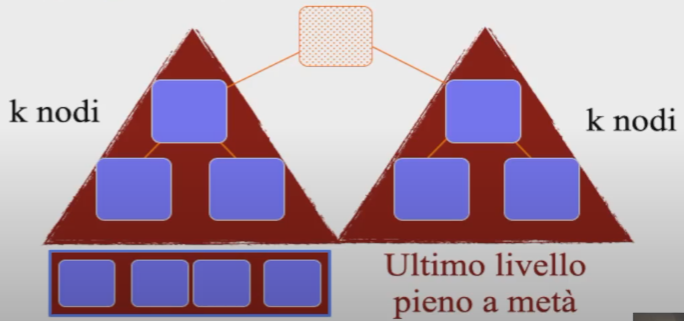
\includegraphics[scale=0.6]{img/costo_maxheapify.png}
        \centering
    \end{figure}
    \item Dato che nell'ultimo livello avrò \verb|k + 1| nodi, i nodi totali dell'albero saranno $n = (2k + 1) + (k + 1) = 3k + 2$.
    \item Dato che il caso peggiore avviene quando si procede verso sinistra dove abbiamo $2k + 1$ nodi, occorre scrivere questo valore in funzione di \verb|n|.
    \item Quindi dato che $n = 3k + 2$, allora $k = (n - 2)/3$.
    \item Adesso sostituisco \verb|k| nel numero di nodi a sinistra e ottengo: $2(n - 2)/3 + 1 = \frac{2}{3} n - \frac{1}{3} < \frac{2}{3} n$.
    \item Quindi dato che a sinistra c'è un numero di nodi inferiore a $\frac{2}{3} n$, l'equazione di ricorrenza al caso peggiore sarà:
    \begin{equation*}
        T(n) = T(2/3 n) + \Theta(1)
    \end{equation*}
    \item Applicando il \verb|Master Theorem| otteniamo $O(\log n)$.
\end{itemize}

\cprotect\subsubsection{Descrizione \verb|Build_Max_Heap()|}

\begin{itemize}
    \item La procedura \verb|Build_Max_Heap()| consente di trasformare un array \verb|A| in un albero di Max-Heap.
    \item Dato che le foglie, se prese singolarmente, sono già degli alberi di Max-Heap, questa funzione chiama la \verb|Max-Heapify| su tutti i nodi interni a partire dall'ultimo nodo non foglia fino alla radice dell'albero generale.
\end{itemize}

\cprotect\subsubsection{Invariante di Ciclo \verb|Build_Max_Heap()|}

All'inizio di ogni iterazione del \verb|for|, ogni nodo $x \in \{i + 1, \dots, n\}$ è radice un Max-Heap. \\
La proprietà viene sempre soddisfatta, anche prima della prima iterazione, perchè i nodi presi in considerazione sono tutte delle foglie che per definizione sono già dei Max-Heap.

\paragraph{Costo}

\begin{itemize}
    \item Quando chiamiamo la \verb|Max-Heapify()|, il suo costo è proporzionale all'altezza del nodo su cui la invochiamo.
    \item Quindi per determinare il costo della \verb|Build-Max-Heap()| occorre calcolare una somma pesata del valore dell'altezza su ogni nodo:
    \begin{equation*}
        T(n) = \sum_{i = 0}^h n_i \cdot h_i
    \end{equation*}
    \item In questa sommatoria, \verb|h| rappresenta l'altezza dell'albero e quindi il numero di livelli che ha, mentre $n_i$ è il numero di nodi al livello \verb|i|, i quali, dato che avranno la stessa altezza possiamo moltiplicare il valore dell'altezza al livello \verb|i| ($h_i$) per il numero di nodi su quel livello.
    \item Ora dato che il numero di nodi su un dato livello \verb|i| è uguale a $2^i$ e l'altezza di un nodo è uguale all'altezza dell'albero meno il livello a cui si trova il nodo ($h_i = h - i$), possiamo sostituire:
    \begin{equation*}
        T(n) = \sum_{i = 0}^h 2^i \cdot (h - i)
    \end{equation*}
    \item Adesso scrivo $2^i$ come $\frac{1}{2^{-i}}$ e moltiplico numeratore e denominatore per $2^h$:
    \begin{equation*}
        T(n) = \sum_{i = 0}^h \frac{h - i}{2^h \cdot 2^{-i}} 2^h = \sum_{i = 0}^h \frac{h - i}{2^{h - i}}2^h
    \end{equation*}
    \item Ora cambio variabile $k = h - i$ e porto $2^h$ fuori dalla sommatoria:
    \begin{equation*}
        \begin{split}
            T(n) & = 2^h \sum_{i = 0}^h \frac{k}{2^k} \\
            & \leq n \sum_{i = 0}^{\infty} \frac{k}{2^k} \\
            & = n \cdot 2 \\
            & = O(n) \\
        \end{split}       
    \end{equation*}
    \item Negli ultimi passaggi abbiamo posto un limite superiore della sommatoria facendola iterare fino ad infinito, quella essendo una sommatoria notevole, il suo valore è $2$ e quindi $T(n) = O(n)$.
\end{itemize}

\cprotect\subsubsection{Descrizione \verb|HeapSort()|}

\begin{enumerate}
    \item All'inizio l'array \verb|A| viene trasformato in un albero di \verb|Max-Heap|.
    \item Successivamente dato che l'elemento più grande si trova nella radice viene posto alla fine dell'array.
    \item La lunghezza dell'Heap (\verb|n|) viene decrementata di 1 perchè nell'ultima cella abbiamo già l'elemento in posizione corretta.
    \item Data che abbiamo inserito in \verb|A[0]| un valore che non sappiamo essere più grande dei suoi sottoalberi, occorre richiamare la \verb|Max_Heapify| di nuovo sull'array ma questa volta solo fino ad \verb|n-1|.
    \item Questa procedura viene eseguita iterativamente fino a quando \verb|i| non raggiunge il valore di 1 (non fino a 0 dato che non ha senso ordinare una porzione di array con solo un elemento).
\end{enumerate}

\subsubsection{Invariante di Ciclo}

All'inizio di ogni \verb|for| la sottoporzione \verb|A[0,...,i]| è un Max-Heap che contiene gli \verb|i| elementi più piccoli di \verb|A| e il sottoarray \verb|A[i+1,...,n]| contiene gli \verb|n-1| elementi più grandi di \verb|A| ordinati.

\lstinputlisting[language=JavaScript]{code/heapsort.js}

\subsection{Counting Sort}

\subsubsection{Descrizione}

\begin{itemize}
    \item L'idea è quella di ordinare un array \verb|A| di \verb|n| elementi dove ogni \verb|A[i]| $\in \{0, 1, 2, \dots, k\}$.
    \item Inizialmente viene istanziato un array \verb|C| di lunghezza \verb|k| dove in posizione \verb|i| saranno contate il numero di occorrenze del numero \verb|i| in \verb|A|.
    \item Infine ogni numero \verb|z| $\in \{0, \dots, k\}$ viene inserito nell'array ordinato \verb|B| per \verb|v| volte.
\end{itemize}

\lstinputlisting[language=JavaScript]{code/counting.js}

\subsection{Radix Sort}

\subsubsection{Descrizione}

\begin{itemize}
    \item L'idea si basa sull'ordinare i numeri decimali per cifre, partentendo dalla meno alla più significativa.
    \item In questo caso conviene utilizzare il \verb|CountingSort()| come algoritmo di ordinamento stabile da che \verb|k| $\in \{0, \dots, 9\}$ (ogni cifra è sempre compresa tra $0$ e $9$).
\end{itemize}

\lstinputlisting[language=JavaScript]{code/radix.js}

\subsection{Ordinamento per Confronti - Lower Bound}

\begin{itemize}
    \item Dati $n$ elementi, il loro ordine corretto di trova in una delle loro $n!$ permutazioni.
    \item Gli ordinamenti per confronti possono essere visti come degli alberi di decisioni, ovvero alberi binari pieni dove ogni nodo contiene una coppia di numeri e a seconda di chi è più grande dell'altro si procede verso destra o verso sinistra.
    \begin{figure}[h]
        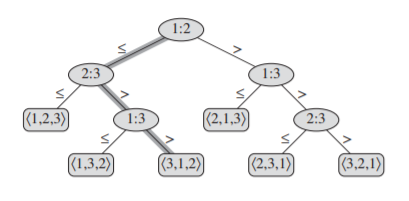
\includegraphics{img/albero_decisionale.png}
        \centering
    \end{figure}
    \item Nell'albero ogni foglia rappresenta una permutazione degli $n$ elementi.
    \item La lunghezza del cammino dalla radice fino alla permutazione che rappresenta l'ordine corretto della sequenza, rappresenta il numero di confronti effettuati dall'algoritmo.
    \item Nel caso peggiore il numero di confronti, e quindi la lunghezza del cammino, è uguale all'altezza $h$ dell'albero binario.
    \item Quindi considerando un albero di decisione di altezza $h$ con $l$ foglie.
    \item Poichè ciascuna delle $n!$ deve comparire in una foglia si ha che $n! \leq l$.
    \item Dato che un un albero di altezza $h$ non ha più di $2^h$ foglie vale la seguente disuguaglianza: $n! \leq l \leq 2^h$.
    \item Applicando la funzione logaritmica a tutti i termini abbiamo che $\log n! \leq \log l \leq h$.
    \item Quindi abbiamo che $h \geq \log n!$.
    \item Per la formula di Stirling $h = \Omega(n \log n)$.
\end{itemize}

$\hfill\blacksquare$

\section{Dimostrazione Master Theorem}

\textbf{\underline{Ipotesi:}} $n$ è una potenza esatta di $b$.

\begin{equation}
    T(n) = aT(n/b) + f(n)
\end{equation}

Data l'equazione di ricorrenza descritta in precedenza, possiamo dire che:

\begin{equation}
    \displaystyle T(n) = \Theta(n^{\log_{b}a}) + \sum_{j = 0}^{\log_{b}n - 1} a^j f(n/b^j)
\end{equation}

Per dimostrare questa uguaglianza occorre utilizzare l'albero di ricorsione associato all'equazione presa in considerazione.

\begin{figure*}[h]
    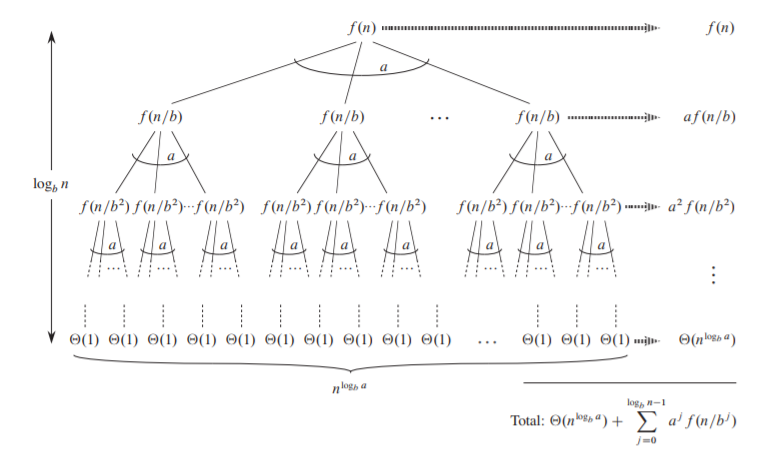
\includegraphics[scale=0.8]{img/albero_master_theorem.png}
    \centering
\end{figure*}

\begin{itemize}
    \item Quindi la radice dell'albero ha costo $f(n)$, e ci sono ogni volta $a$ chiamate ricorsive ($a$ sottoproblemi, ognuno dal costo di $f(n/b)$).
    \item Generalizzando possiamo dire che ogni livello ha costo $a^j f(n/b^j)$.
    \item L'altezza dell'albero è ovviamente $\log_{b} n$, e il numero di foglie sarà uguale a $a^{\log_{b} n}$.
    \item Utilizzando le proprietà dei logaritmi abbiamo che $a^{\log_{b} n} = n^{\log_{b} a}$.
    \item Quindi se vogliamo calcolare il costo complessivo dell'albero, possiamo sommare il costo delle foglie che hanno tutte costo $\Theta(1)$. Quindi $\Theta(1) \cdot \Theta(n^{\log_{b} a}) = \Theta(n^{\log_{b} a})$.
    \item E a questo valore possiamo sommare il costo di ogni livello, a partire dalla radice ($j = 0$) fino al penultimo livello dell'albero ($\log_{b} n - 1$).
\end{itemize}

Adesso occorre dimostrare i 3 casi del Master Theorem.

\subsection{Caso 1}

Dimostrare che:

\begin{equation*}
    f(n) = O(n^{\log_{b}a - \epsilon}) \Rightarrow g(n) = \sum_{j = 0}^{\log_{b}n - 1} a^j f(n/b^j) = O(n^{\log_{b}a})
\end{equation*}

\begin{itemize}
    \item Quindi se sappiamo che $f(n) = O(n^{\log_{b}a - \epsilon})$, allora $f(n/b^j) = O((n/b^j)^{\log_{b}a - \epsilon})$.
    \item $g(n)$ quindi diventa: $\displaystyle g(n) = O(\sum_{j = 0}^{\log_{b}n - 1} a^j(n/b^j)^{\log_{b} a - \epsilon})$.
    \item Adesso posso tirare tutto ciò che non dipende da $j$ fuori dalla sommatoria: $\displaystyle g(n) = \sum_{j = 0}^{\log_{b}n - 1} a^j(\frac{n}{b^j})^{\log_{b} a - \epsilon} = n^{\log_{b}a - \epsilon} \sum_{j = 0}^{\log_{b}n - 1} a^j(\frac{1}{b^j})^{\log_{b} a - \epsilon}$.
    \item Ora utilizzando le proprietà delle potenze possiamo portare $j$ fuori dalle parentesi e portiamo dentro l'esponente che si trova fuori dalle parentesi e lo spezziamo, dividendo il logaritmo con $\epsilon$: $\displaystyle g(n) = n^{\log_{b}a - \epsilon} \sum_{j = 0}^{\log_{b}n - 1} a^j (\frac{b^{\epsilon}}{b^{\log_{b}a}})^j$.
    \item Adesso possiamo semplificare il denominatore all'interno della sommatoria: $\displaystyle g(n) = n^{\log_{b}a - \epsilon} \sum_{j = 0}^{\log_{b} n - 1} a^j (\frac{b^{\epsilon \cdot j}}{a^j})$.
    \item A questo punto semplifichiamo $a^j$: $\displaystyle g(n) = n^{\log_{b}a - \epsilon} \sum_{j = 0}^{\log_{b} n - 1} (b^{\epsilon})^j$.
    \item Per semplificare la sommatoria possiamo utilizzare la seguente serie geometrica: $\displaystyle \sum_{k = 0}^n x^k = \frac{x^{n + 1} - 1}{x - 1}$.
    \item Quindi: $g(n) = n^{\log_{b}a - \epsilon} (\frac{b^{\epsilon \log_{b} n} - 1}{b^{\epsilon} - 1})$.
    \item Ora di nuovo applicando le proprietà dei logaritmi abbiamo che: $g(n) = n^{\log_{b}a - \epsilon} (\frac{n^{\epsilon} - 1}{b^{\epsilon} - 1})$.
    \item Adesso dato che $b$ ed $\epsilon$ sono costanti possiamo riscrivere l'equazione in questo modo: $g(n) = n^{\log_{b}a - \epsilon} \; O(n^{\epsilon})$.
    \item Come ultimo passaggio possiamo portare tutto dentro l'$O$-grande ed eliminare $\epsilon$: $g(n) = O(n^{\log_{b}a - \epsilon + \epsilon}) = O(n^{\log_{b} a})$.
    \item Quindi $g(n) = O(n^{\log_{b} a})$.
\end{itemize}

Adesso effettuando le opportune sostituzioni abbiamo che:

\begin{equation*}
    T(n) = \Theta(n^{\log_{b}a}) + O(n^{\log_{b} a}) = \Theta(n^{\log_{b} a})
\end{equation*}

\subsection{Caso 2}

Dimostrare che:

\begin{equation*}
    f(n) = \Theta(n^{\log_{b}a}) \Rightarrow g(n) = \sum_{j = 0}^{\log_{b}n - 1} a^j f(n/b^j) = \Theta(n^{\log_{b} a} \lg n)
\end{equation*}

\begin{itemize}
    \item Se sappiamo che $f(n) = \Theta(n^{\log_{b} a})$, allora $f(n/b^j) = \Theta((n/b^j)^{\log_{b} a})$.
    \item $g(n)$ quindi diventa: $\displaystyle g(n) = \Theta(\sum_{j = 0}^{\log_{b}n - 1} a^j(\frac{n}{b^j})^{\log_{b} a})$.
    \item Ora portiamo fuori ciò che non dipende da $\displaystyle j$: $\displaystyle g(n) = n^{\log_{b} a} \sum_{j = 0}^{\log_{b}n - 1} (\frac{a}{b^{\log_b a}})^j$.
    \item Adesso applicando le proprietà delle potenze abbiamo che: $\displaystyle g(n) = n^{\log_{b} a} \sum_{j = 0}^{\log_{b}n - 1} 1$.
    \item Quindi calcolando la serie abbiamo che: $g(n) = \Theta(n^{\log_{b} a} \log_{b} n)$.
\end{itemize}

Adesso effettuando le opportune sostituzioni abbiamo che:

\begin{equation*}
    T(n) = \Theta(n^{\log_{b}a}) + \Theta(n^{\log_{b} a} \lg n) = \Theta(n^{\log_{b} a} \lg n)
\end{equation*}

\subsection{Caso 3}

Dimostrare che:

\begin{equation*}
    a f(n/b) \leq c f(n) \Rightarrow g(n) = \sum_{j = 0}^{\log_{b}n - 1} a^j f(n/b^j) = \Theta(f(n))
\end{equation*}

\begin{itemize}
    \item Riscriviamo $f(n)$ dividendo la disequazione per $a$: $f(n/b) \leq (c/a) f(n)$.
    \item Successivamente iteriamo la disequazione per $j$ volte: $f(n/b^j) \leq (c/a)^j f(n)$.
    \item Adesso moltiplichiamo per $a^j$: $a^j f(n/b^j) \leq c^j f(n)$.
    \item A questo punto possiamo effettuare il passaggio alla serie: $\displaystyle g(n) = \sum_{j = 0}^{\log_{b} n - 1} a^j f(n/b^j) \leq \sum_{j = 0}^{\log_{b} n - 1} c^j f(n) + O(1)$.
    \item Possiamo riscrivere la disequazione in questo modo: $\displaystyle g(n) = \sum_{j = 0}^{\log_{b} n - 1} a^j f(n/b^j) \leq \sum_{j = 0}^{\infty} c^j f(n) + O(1)$.
    \item Adesso è possibile calcolare il valore della serie: $\displaystyle g(n) = \sum_{j = 0}^{\log_{b} n - 1} a^j f(n/b^j) \leq f(n) (\frac{1}{1 - c}) + O(1)$.
    \item Dato che $c$ è una costante: $\displaystyle g(n) = \sum_{j = 0}^{\log_{b} n - 1} a^j f(n/b^j) = O(f(n))$.
\end{itemize}

Adesso effettuando le opportune sostituzioni abbiamo che:

\begin{equation*}
    T(n) = \Theta(n^{\log_{b}a}) + \Theta(f(n)) = \Theta(f(n))
\end{equation*}

Questo perchè nelle ipotesi del Caso 3 abbiamo che $f(n) = \Omega(n^{\log_{b}a + \epsilon})$.

\section{Algoritmi di Ricerca}

\subsection{Ricerca Lineare}

\lstinputlisting[language=JavaScript]{code/linear_search.js}

\subsection{Ricerca Binaria}

\lstinputlisting[language=JavaScript]{code/binary_search.js}

\section{Tabelle Hash}

\subsection{Gestione delle Collisioni}

\begin{center}
    \begin{tabular}{|c|c|c|c|}
        \hline
        & \multicolumn{3}{c|}{Operazione} \\
        \hline
        Gestione & Inserimento & \makecell{Ricerca con \\ successo} & \makecell{Ricerca senza \\ successo} \\ \hline     
        \makecell{Liste di \\ Trabocco} & $O(1)$ & $\Theta(1 + \alpha)$ & $\Theta(1 + (1 + \frac{\alpha}{2} - \frac{\alpha}{2n}))$ \\ \hline
        Open Hash & \makecell{$T_{ottimo} = \Theta(1)$ \\ $T_{pessimo} = \Theta(n) = \Theta(m)$ \\ $T_{medio} = O(\frac{1}{1 - \alpha})$} & $O(\frac{1}{\alpha} \ln (\frac{1}{1 - \alpha}))$ & $O(\frac{1}{1 - \alpha})$ \\ \hline
    \end{tabular}
\end{center}

\subsection{Liste di Trabocco}

\begin{theorem}[Ricerca senza Successo - Caso Medio]
    In una tabella hash con concatenamento la ricerca senza successo richiede al caso medio $\Theta(1 + \alpha)$, dove $\alpha = \frac{n}{m}$.
\end{theorem}

\begin{proof}
    $ $\newline
    \begin{itemize}
        \item Definiamo $\alpha = \frac{\abs{S}}{dim \; T} = \frac{n}{m}$ come il fattore di carico.
        \item Data la chiave \verb|k|, effettuo l'hashing \verb|h(k)| e verifico se in testa alla lista \verb|T[h(k)]| è presente la chiave cercata.
        \item Se in testa non è presente, occerrerà scorrere tutta la lista.
        \item Se gli \verb|n| elementi sono distribuiti uniformemente sulle liste, ogni lista conterrà $\alpha$ elementi.
        \item Quindi $T_{medio}(n, m) = \Theta(1 + \alpha)$, dove l'$1$ è dovuto al calcolo di \verb|h(k)| e $\alpha$ al numero di ispezioni nella lista.
        \item Se $\alpha$ è costante allora: $T_{medio}(n, m) = \Theta(1)$.
    \end{itemize}
\end{proof}

\begin{theorem}[Ricerca con Successo - Caso Medio]
    In una tabella hash con concatenamento la ricerca con successo richiede al caso medio $\Theta(1 + (1 + \frac{\alpha}{2} - \frac{\alpha}{2n})) = \Theta(1 + \alpha)$, dove $\alpha = \frac{n}{m}$. 
\end{theorem}

\begin{proof}
    $ $\newline
    \begin{itemize}
        \item Il numero di ispezioni per trovare \verb|k| è dovuto dal numero di elementi che precedono \verb|k| nella lista \verb|T[h(k)]|. Essendoci l'inserimento in testa, questi sono gli elementi inseriti dopo \verb|k|.
        \item Se \verb|x| è l'i-esimo elemento, quelli inseriti dopo sono \verb|n - i| elementi.
        \item Gli elementi, invece, che avranno lo stesso valore hash \verb|h(k)| saranno in media $\lfloor \frac{n - i}{m} \rfloor$.
        \item Quindi gli elementi ispezionati durante la ricerca di \verb|i| sono $1 + \frac{n - i}{m}$.
        \item A questo punto occorre fare una media su tutte le posizioni che può assumere \verb|i| nella lista; quindi supponiamo che stiamo cercando uno degli elementi con la stessa probabilità $1/n$.
        \item Quindi il numero di ispezioni al caso medio è uguale a:
            \begin{equation*}
                \frac{1}{n} \sum_{i = 1}^n (1 + \frac{n - i}{m}) = \frac{1}{n} \sum_{i = 1}^n 1 + \frac{1}{n} \sum_{i = 1}^n \frac{n - i}{m} =
            \end{equation*}
        \item La prima sommatoria è uguale a $n$ e possiamo portare fuori dalla seconda sommatoria $m$:
            \begin{equation*}
                = \frac{n}{n} + \frac{1}{n \cdot m} \sum_{i = 1}^n (n - i) =
            \end{equation*}
        \item Adesso possiamo notare che la sommatoria rimasta corrisponde alla somma dei primi $n$ numeri interi (formula di Gauss), quindi:
            \begin{equation*}
                = 1 + \frac{1}{n \cdot m} \cdot \frac{n(n-1)}{2} = 1 + \frac{n - 1}{2m} = 1 + \frac{n}{2m} - \frac{1}{2m} =
            \end{equation*}
        \item Dato che $\alpha = \frac{n}{m}$ e $m = \frac{n}{\alpha}$:
            \begin{equation*}
                = 1 + \frac{\alpha}{2} - \frac{\alpha}{2n}
            \end{equation*}
    \end{itemize}
\end{proof}

\subsection{Open Hash}

\textbf{\underline{Ipotesi:}}

\begin{enumerate}
    \item $\alpha = \frac{n}{m} < 1$.
    \item Non sono previste cancellazioni.
    \item Deve valere l'ipotesi di Hashing Uniforme (la sequenza di ispezione deve essere una permutazione generata con pari probabilità).
\end{enumerate}

\begin{theorem}[Ricerca senza Successo - Caso Medio]
    In una tabella hash a indirizzamento aperto, la ricerca senza successo effettua, al caso medio, un numero di accessi $\leq \frac{1}{1 - \alpha}$.
\end{theorem}

\begin{proof}
    $ $\newline
    \begin{itemize}
        \item Poniamo \verb|X| come il numero di accessi alla tabella per effettuare la nostra ricerca.
        \item Il valore medio di \verb|X| è uguale alla somma di tutti i valori che può assumere, moltiplicato per la probabilità che \verb|X| assuma quel valore:
            \begin{equation*}
                \sum_{i = 1}^{\infty} i \cdot Prob[x = i] = \sum_{i = 1}^{\infty} Prob[x \geq i]
            \end{equation*}
        \item Nel passaggio precedente la serie è stata semplificata, e a questo punto ci ritroviamo con la probabilità che \verb|X| effettui almeno \verb|i| accessi:
            \begin{itemize}
                \item[-] Se $i = 1$, $Prob[x \geq 1] = 1$.
                \item[-] Se $i = 2$, $Prob[x \geq 2] = \alpha$. Essenzialmente è la probabilità di trovare la prima cella già occupata da una chiave diversa ma con lo stesso \verb|h(k)|.
                \item[-] Se $i = 3$, $Prob[x \geq 3] = \frac{n}{m} \cdot \frac{n - 1}{m - 1} \leq \alpha^2$. Quindi la probabilità di avere sia la prima che la seconda cella già occupata).
            \end{itemize}
        \item Quindi generalizzando:
            \begin{equation*}
                \sum_{i = 1}^{m} Prob[x \geq i] = \sum_{i = 1}^{m} \alpha^{i - 1} = \sum_{i = 0}^{m - 1} \alpha^i \leq \sum_{i = 1}^{\infty} \alpha^i =
            \end{equation*}
        \item L'ultima sommatoria è una serie geometrica, quindi essendo $\alpha \leq 1$:
            \begin{equation*}
                = \frac{1}{1 - \alpha}
            \end{equation*}
    \end{itemize}
\end{proof}

\begin{theorem}[Ricerca con Successo - Caso Medio]
    In una tabella hash a indirizzamento aperto, la ricerca con successo effettua, al caso medio, un numero di accessi $\leq \frac{1}{\alpha} \cdot \ln(\frac{1}{1 - \alpha})$.
\end{theorem}

\begin{proof}
    $ $\newline
    \begin{itemize}
        \item Chiamiamo \verb|k| la chiave che stiamo cercando; \verb|k| è l'i-esimo elemento inserito nella tabella.
        \item Se chiamiamo $\alpha_i$ il fattore di carico nella tabella prima dell'inserimento di \verb|k|:
            \begin{equation*}
                \alpha_i = \frac{i}{m}
            \end{equation*}
        \item Quindi il numero di accessi fatti per inserire \verb|k| è uguale al numero di accessi per una ricerca senza successo:
            \begin{equation*}
                \leq \frac{1}{1 - \alpha_i} = \frac{1}{1 - \frac{i}{m}} = \frac{m}{m - i}
            \end{equation*}
        \item Quindi il valore medio del numero di accessi è:
            \begin{equation*}
                \frac{1}{n} \sum_{i = 0}^{n - 1} \alpha_i = \frac{1}{n} \sum_{i = 0}^{n - 1} \frac{m}{m - i} = \frac{m}{n} \sum_{i = 0}^{n - 1} \frac{1}{m - i} =
            \end{equation*}
        \item Adesso per calcolare il valore della serie possiamo applicare il Criterio dell'Integrale:
            \begin{equation*}
                = \frac{1}{\alpha} \sum_{i = 0}^{n - 1} \frac{1}{m - i} \leq \frac{1}{\alpha} \cdot \int_{m - n}^m \frac{1}{x} \; dx = \frac{1}{\alpha} \cdot \ln(\frac{m}{m - n}) =
            \end{equation*}
        \item A questo punto occorre solo dividere il numeratore e il denominatore del logaritmo per $m$:
            \begin{equation*}
                = \frac{1}{\alpha} \cdot \ln(\frac{1}{1 - \alpha})
            \end{equation*}
    \end{itemize}
\end{proof}

\section{2-3 Alberi}

\begin{lemma}
    Dato un 2-3 Albero alto h, con n nodi e con f foglie, vale che:
    \begin{equation*}
        2^{h+1}-1 \leq n \leq (3^{h+1} - 1) / 2
    \end{equation*}
    \begin{equation*}
        2^h \leq f \leq 3^h
    \end{equation*}
\end{lemma}

\begin{proof}
    Poniamo $T$ come un albero alto $h + 1$, e $T'$ come l'albero alto $h$ ottenuto eliminando da $T$ tutte le foglie. \\
    Adesso dimostriamo la seguente Ipotesi Induttiva:
    \begin{equation*}
        2^{h+1}-1 \leq n' \leq (3^{h+1} - 1) / 2
    \end{equation*}
    \begin{equation*}
        2^h \leq f' \leq 3^h
    \end{equation*}
    Dato che ogni foglia in $T'$ ha o 2 o 3 figli in $T$ risulta che:
    \begin{equation*}
        2 \cdot 2^h \leq f \leq 3 \cdot 3^h
    \end{equation*}
    \begin{equation*}
        2^{h+1} \leq f \leq 3^{h+1}
    \end{equation*}
    Come ultimo passo sappiamo che il numero di nodi in $T$ è uguali al numero di nodi in $T'$ più il numero di foglie in $T$, quindi:
    \begin{equation*}
        2^{h+1}-1 + 2^{h+1} \leq n' + f \leq (3^{h+1}-1) / 2 + 3^{h+1}
    \end{equation*}
    \begin{equation*}
        2^h(2 + 2) - 1 \leq n \leq (3^{h+1}-1 + 2 \cdot 3^{h+1}) / 2
    \end{equation*}
    \begin{equation*}
        2^{h+2} - 1 \leq n \leq [3^h(3 + 2 \cdot 3) - 1] / 2
    \end{equation*}
    \begin{equation*}
        2^{h+2} - 1 \leq n \leq (3^{h+2} - 1) / 2
    \end{equation*}
\end{proof}

\section{Programmazione Dinamica}

\subsection{LCS}

\begin{theorem}[Sottostruttura ottima delle LCS]
    Date due stringhe $X = x_1, \cdots, x_m$ e $Y = y_1, \cdots, y_n$ e una stringa
    $Z = z_1, \cdots, z_k$ tale che $Z = LCS(X, Y)$:
    \begin{enumerate}
        \item $x_m = y_m \Rightarrow z_k = x_m = y_n$ e $Z_{k-1}$ è $LCS(X_{m-1}, Y_{n-1})$.
        \item $x_m \neq y_m \Rightarrow z_k \neq x_m$ e $Z$ è $LCS(X_{m-1}, Y_{n})$.
        \item $x_m \neq y_m \Rightarrow z_k \neq y_n$ e $Z$ è $LCS(X_{m}, Y_{n-1})$.
    \end{enumerate}
\end{theorem}

\begin{proof}
    $ $
    \begin{enumerate}
        \item Se per assurdo $z_k \neq x_m$ ma $x_m = y_n$ allora possiamo accodare $x_m$ a $Z$ per ottenere
            una sottosequenza comune di X e Y lunga $k+1$ contraddicendo l'ipotesi che $Z$ sia una LCS di X e Y. \\
            Ora dimostriamo che $Z_{k-1} = LCS(x_{m-1}, y_{n-1})$ lunga $k - 1$. Supponiamo che esista una stringa
            chiamata $W$ che è una sottosequenza comune di $X_{m-1}$ e $Y_{n-1}$ di lunghezza maggiore di $k - 1$. Allora
            accodando $x_m = y_n$ a $W$ si otterrebbe una sottosequenza di lunghezza maggiore di $k$, ma questo contraddice
            l'ipotesi $Z = LCS(X, Y)$.
        \item Se esistesse una stringa $W$ sottosequenza comune di $X_{m-1}$ e $Y$ di lunghezza maggiore di $k$, allora
            $W$ sarebbe anche una sottosequenza comune di $X$ e $Y$ (questo perchè $x_m \neq y_n$), ma questo contraddice l'ipotesi
            $Z = LCS(X, Y)$.
        \item La dimostrazione è simmetrica al punto 2.
    \end{enumerate}
\end{proof}

\section{Grafi}

\subsection{Dimostrazione Calcolo Cammino Minimo BFS}

\begin{lemma}
    Dato un grafo G = (V, E) e una sorgente $s \in V$, per ogni arco $(u, v) \in E$, 
    $\delta(s, v) \leq \delta(s, u) + 1$, questo perchè la distanza tra s e v è sicuramente minore 
    o uguale a qualsiasi altro cammino da s a v; in questo caso un cammino che da s va in u e tramite l'arco (u, v) arriva in v. 
\end{lemma}

\begin{lemma}
    Al termine dell'algoritmo \verb|BFS(G, s)|, per ogni vertice $v \in V$, $v.d \geq \delta(s, v)$.
\end{lemma}

\begin{proof}
    Poniamo la seguente Ipotesi Induttiva: $v.d \geq \delta(s, v)$. \\
    \begin{enumerate}
        \item[\textbf{1)}] \textbf{Caso Base} \\
        $s.d = 0 = \delta(s, s)$ \\
        $v.d = \infty \geq \delta(s, v)$ per ogni $v \in V$\textbackslash$\{s\}$ \\
        Queste uguaglianze ovviamente sono vere dopo la \verb|Enqueue(Q, s)| nella \verb|BFS(G, s)|.
        \item[\textbf{2)}] \textbf{Passo Induttivo} \\
        Se v è un vertice bianco scoperto da u, dimostriamo che l'ipotesi Induttiva è sempre valida: \\
        \begin{equation*}
            \begin{split}
                v.d & = u.d + 1 \; \text{(Questo è l'assegnamento che esegue l'algoritmo).} \\
                & \geq \delta(s, u) + 1 \; \text{(per Ipotesi Induttiva).} \\
                & \geq \delta(s, v) \; \text{(Per il Lemma 7.1).} \\
            \end{split}
        \end{equation*}
        A questo punto questa disuguaglianza è sempre verificata dato che v.d non cambia più perchè il vertice diventa grigio. 
    \end{enumerate}
\end{proof}

\begin{lemma}
    Durante la BFS, se $Q = [v_1, v_2, \dots, v_r]$, allora:
    \begin{enumerate}
        \item $v_r.d \leq v_1.d + 1$ (la differenza tra $v_1$ e $v_r$ è 1).
        \item $v_i.d \leq v_{i + 1}.d \; \forall \; i \in \{1, 2, \dots, r - 1\}$.
    \end{enumerate}
    Questo significa che, in ogni istante, nella coda ci sono al più 2 valori diversi della distanza dalla sorgente, e i campi distanza formano una successione crescente.
\end{lemma}

\begin{corollary}
    I valori delle distanze dalla sorgente, dei vertici inseriti nella coda, sono monotoni crescenti, quindi se $v_i$ è inserito nella coda prima di $v_j$, allora $v_i.d \leq v_j.d$.
\end{corollary}

\begin{theorem}
    La BFS scopre tutti i vertici $v \in V$ raggiungibili dalla sorgente s e alla fine dell'algoritmo, 
    $v.d = \delta(s, v)$ per ogni $v \in V$. \\
    Inoltre per ogni $v \neq s$, raggiungibile da s, uno dei cammini minimi da s a v è un cammino minimo da s a $v.\pi$ seguito dall'arco $(v.\pi, v)$.
\end{theorem}

\begin{proof}
    Supponiamo che ci sia un vertice v che è il nodo più vicino alla sorgente che ha il campo "d" diverso dalla sua distanza dalla sorgente. \\ \\
    Per il Lemma 7.2, $v.d \geq \delta(s, v)$, e dato che abbiamo appena posto che v.d deve essere diverso dalla distanza, allora $v.d > \delta(s, v)$. \\
    Inoltre v deve essere per forza raggiungibile dalla sorgente, altrimenti $\delta(s, v) = \infty \geq v.d$. \\ \\
    Poi, sia u il nodo che precede v in un cammino minimo da s a v, quindi:
    \begin{itemize}
        \item $\delta(s, v) = \delta(s, u) + 1$.
        \item $\delta(s, u) \leq \delta(s, v)$ e $u.d = \delta(s, u)$. Quest'ultima uguaglianza è vera perchè 
        abbiamo posto che v è il nodo più vicino alla sorgente con il campo v.d errato, quindi il campo u.d sarà corretto perchè u si trova prima di v.
    \end{itemize}
    Dunque mettendo insieme i pezzi possiamo dire che: $v.d > \delta(s, v) = \delta(s, u) + 1 = u.d + 1$ e quindi \underline{$v.d > u.d + 1$}. \\
    Quando u viene estratto dalla coda, v può essere di colore bianco, grigio o nero:
    \begin{enumerate}
        \item Se v è bianco, allora l'algoritmo assegna \underline{$v.d = u.d + 1$}. \lightning
        \item Se v è nero, allora v era stato già rimosso dalla coda e per il Corollario 7.1 \underline{$v.d \leq u.d$}. \lightning
        \item Se v è grigio, allora v è stato scoperto da un vertice w estrato dalla coda Q prima di u e quindi v.d = w.d + 1. \\
        Per il Corollario 7.1 $w.d \leq u.d$, quindi $v.d = w.d + 1 \leq u.d + 1$, \underline{$v.d \leq u.d + 1$}. \lightning
    \end{enumerate}
    \begin{center}
        Quindi $v.d = \delta(s, v)$.
    \end{center}
    Infine, tutti i vertici raggiungibili da s devono essere scoperti, altrimenti $\infty = v.d > \delta(s, v)$.
\end{proof}

\subsection{DFS - Visita in Profondità}

\subsubsection{Proprietà Foresta DF}

\begin{enumerate}
    \item u è il padre di v in un albero della foresta DF $\Leftrightarrow$ v è stato scoperto esaminando la lista di adiacenza di u.
    \item v è discendente di u nella foresta DF $\Leftrightarrow$ v è stato scoperto quando u era Grigio.
\end{enumerate}

\subsection{Teoremi Principali}

\begin{theorem}[Teorema delle Parentesi]
    Dati gli intervalli $I_u = [u.d, u.f]$ e $I_v = [v.d, v.f]$, $\forall \; u, v \in V$ è soddisfatta una sola delle seguenti tre condizioni:
    \begin{enumerate}
        \item $I_u \cap I_v = \varnothing \Rightarrow$ u e v non sono discendenti uno dell'altro.
        \item $I_v \subset I_u \Rightarrow$ v è discendente di u.
        \item $I_u \subset I_v \Rightarrow$ u è discendente di v.
    \end{enumerate}
\end{theorem}

\begin{proof}
    Per ipotesi poniamo $u.d < v.d$. Ci possono essere 2 casi:
    \begin{enumerate}
        \item $u.f < v.d \Rightarrow u.d < u.f < v.d < v.f \Rightarrow I_u \cap I_v = \varnothing$.
        \item $u.f > v.d \Rightarrow$ v è stato scoperto quando quando u era Grigio, quindi v è un discendente di u $\Rightarrow$ la visita di v termina prima di quella di u $\Rightarrow I_v \subset I_u$.  
    \end{enumerate}
    La dimostrazione è speculare nel caso $v.d < u.d$.
\end{proof}

\begin{corollary}[Corollario di Annidamento degli Intervalli]
    v è discendente di u nella foresta DF ($u \neq v$) $\Leftrightarrow I_v \subset I_u$.
\end{corollary}

\begin{theorem}[Teorema del Cammino Bianco]
    v è un discendente di u nella foresta DF $\Leftrightarrow$ al tempo u.d, v può essere raggiunto da u lungo un cammino di soli vertici Bianchi.
\end{theorem}

\begin{proof}
    $ $
    \begin{itemize}
        \item[$\Rightarrow$]$ $
            \begin{itemize}
                \item[$v = u$] In questo caso il cammino $u \leadsto v$ contiene solo il nodo u che è Bianco al tempo u.d.
                \item[$v \neq u$] v è un discendente diretto di u. Per il Corollario 7.2 se $I_v \subset I_u$ allora $u.d < v.d$. Quindi v è scoperto dopo u, e per questo v è Bianco all'istante u.d. Se v non è un discendente diretto di u, applicando in modo induttivo il ragionamento precedente su tutti i vertici lungo l'unico cammino nella foresta DF da u a v, essi saranno tutti Bianchi al tempo u.d.
            \end{itemize} 
        \item[$\Leftarrow$] Per assurdo diciamo che esiste un cammino Bianco $u \leadsto v$ al tempo u.d, ma che v non è discendente di u.
            Scegliamo v come il vertice più vicino a u che non è discendente di u. Inoltre scegliamo w come il vertice che precede direttamente v sul cammino.
            w è discendente di u, quindi $I_w \subseteq I_u$ e $w.f \leq u.f$ (w e u possono essere lo stesso vertice). Inoltre sappiamo che v è Bianco al tempo u.d. Quindi: \\
            $u.d < v.d < w.f \leq u.f$. Il primo '$<$' è vero perchè v è Bianco al tempo u.d. Il secondo '$<$', invece, è vero perchè $v \in Adj[w]$, quindi la visita di w è ancora in corso quando v viene scoperto.
            Il terzo '$\leq$' è vero perchè w è discendente di u. \\
            Per il Teorema delle Parentesi, dato che $v.f < u.f$, allora $I_v \subset I_u$ e v è discendente di u. \lightning
    \end{itemize}
\end{proof}

\subsection{Archi}

\begin{theorem}
    In una DFS su un grafo non orientato, gli archi sono solo archi d'albero e archi all'indietro.
\end{theorem}

\begin{proof}
    $(u, v) \in E$. Supponiamo che sia stato scoperto prima u, allora $u.d < v.d$. Quindi v diventa Grigio e successivamente Nero, invece u è Grigio. Ci sono 2 casi:
    \begin{enumerate}
        \item (u, v) è esplorato la prima volta da u verso v, allora v è Bianco e (u, v) diventa arco d'albero.
        \item (u, v) è esplorato la prima volta da v verso u, allora u è Grigio e (u, v) è un arco all'indietro.
    \end{enumerate}
\end{proof}

\begin{theorem}
    Un grafo G è ciclico $\Leftrightarrow$ G contiene almeno un arco all'indietro.
\end{theorem}

\begin{proof}
    $ $
    \begin{itemize}
        \item[$\Leftarrow$] (u, v) è un arco all'indietro di un grafo orientato o non orientato e v è un antenato di u. Il cammino $v \leadsto u$ in un albero DF, unito all'arco (u, v) forma un ciclo.
        \item[$\Rightarrow$] Se il grafo non è orientato, gli archi di un ciclo non possono tutti essere d'albero, quindi ci dev'essere almeno un arco all'indietro. \\
        Se il grafo è orientato, poniamo v come il primo vertice di un ciclo ad essere scoperto e che diventa Grigio, allora quando si scopre v, gli altri nodi sono Bianchi. Poniamo u, invece, come il nodo che precede v nel ciclo.
        Al tempo v.d tutti i vertici sul cammino $v \leadsto u$ sono Bianchi. \\
        Per il Teorema del Cammino Bianco, u diventa un discendente di v, quindi v è un antenato di u e (u, v) è un arco all'indietro. 
    \end{itemize}
\end{proof}

\subsection{Ordinamento Topologico}

\begin{theorem}
    $\forall \; (u, v) \in E$, se u precede v nell'ordinamento, allora u deve precedere v nella lista; quindi
    u deve essere inserito in lista dopo v. Affinchè questo avvenga, $u.f > v.f$.
\end{theorem}

\begin{proof}
    Quando si ispeziona l'arco (u, v), (u è Grigio), ci sono 3 casi:
    \begin{enumerate}
        \item Se v è Bianco, allora (u, v) è un arco d'albero, quindi v è discendente di u e $v.f < u.f$.
        \item Se v è Nero, allora la visita di v è già finita, mentre quella di u è ancora in corso, quindi $v.f < u.f$.
        \item Se v è Grigio, allora G contiene un ciclo, ma questo è impossibile perchè G deve essere un DAG.
    \end{enumerate}
\end{proof}

\end{document}